%\documentclass[a4paper,twocolumn]{report}
\documentclass[a4paper,twocolumn]{scrartcl}
\addtokomafont{sectioning}{\rmfamily}
\usepackage[utf8]{inputenc}
\usepackage[ngerman]{babel}
\usepackage[left=1.5cm,right=1.5cm,top=2cm,bottom=2cm]{geometry}
\setlength{\columnsep}{5ex}
\usepackage{enumitem}
\usepackage{amsmath}
\usepackage{amssymb}
\usepackage[pdftex]{graphicx}
\usepackage{color}
    \definecolor{lightgray}{gray}{.95}
\usepackage{listings}
    \lstset{
    %basicstyle=\usefont{T1}{pcr}{m}{n}\small, 
    %basicstlye=\small,
    numbers=none,
    numberstyle=\tiny,
    numbersep=5pt,
    backgroundcolor=\color{lightgray},
    showspaces=false,
    showstringspaces=false,
    showtabs=false, 
    frame=tb, 
    framerule=.8pt, 
    rulecolor=\color{black}, 
    tabsize=2,
    captionpos=b,
    breaklines=true,
    breakatwhitespace=true,
    title=\lstname,
    keywordstyle=\bfseries,
    stringstyle=\usefont{T1}{pcr}{m}{sl}\small,
    escapeinside={@}{@},
    morekeywords={process,in,out,is,begin,for,do,if,then, else, end, while}
    }
\newcommand{\lststyle}[1]{{\usefont{T1}{pcr}{m}{n}\small\selectfont#1}}

\author{Julian Dobmann, Frederik Feiten, Felix Herter, Johannes Sauer}
\title{Softwareprojekt Anwendung von Algorithmen}
\subtitle{Punkte in allgemeiner Lage}
 

\begin{document}

\twocolumn[
  \begin{@twocolumnfalse}
  \maketitle
  \vspace{-5ex}
  \rule{\textwidth}{1pt}
    \begin{abstract}
    \textbf{
      Bacon ipsum dolor sit amet meatloaf id ball tip anim sunt, corned beef ad pork loin prosciutto non velit ut nisi deserunt. Eu beef ex tri-tip meatball in pork chop, officia drumstick proident laborum. Aute short loin spare ribs corned beef. Proident labore kielbasa ham hock sint ut, fugiat nisi prosciutto chuck chicken. Pig fugiat bresaola, ut strip steak boudin proident officia. Elit andouille pork chop ut cow adipisicing short loin, in et laborum dolore in.}
    \end{abstract}
  \end{@twocolumnfalse}
]

\tableofcontents

\section{Einleitung}

\section{Datenstrukturen}

\subsection{Einführung der arithmetischen Unschärfe}
Bedingt durch die endliche Darstellung von Flie\ss kommazahlen im Prozessor waren wir gezwungen eine arithmetische
Unsch\"arfe einzuf\"uhren. \\
Wird zum Beispiel der Ausdruck $0.3-0.1$ berechnet, so wird anstelle des exakten Ergebnisses von $0.2$ 
als n\"achstbeste  Näherung:
\begin{lstlisting}
js> 0.3-0.1
0.19999999999999998
\end{lstlisting}
zur\"uckgeliefert. Die Differenz des exakten Wertes von der N\"aherung bel\"auft sich auf
\begin{lstlisting}
js> 0.2-(0.3-0.1)
2.7755575615628914e-17
\end{lstlisting}
, weicht also um die Gr\"o\ss enordung $10^{-16}$ von der, der Operanden ab.
Wir haben uns entschienden die arithmetische Unsch\"arfe auf $10^{-10}$ zu setzen. (\textbf{(remove me) Warum?}).
\subsection{Punkte und Vektoren}
Als grundlegende Datenstruktur wurden Vektoren eingef\"uhrt. Diese haben ihre zwei kartesischen Koordinaten als
Attribute und verf\"ugen \"uber die grundlegenden Eigenschaften und Funktionalit\"aten, welche von ihnen zu erwarten sind
(Vektoraddition/-subtraktion,
Multiplikation mit einem Skalar, Skalarmultiplikation, etc.). \textbf{(remove me) explizit dokumentieren}\\
Ohne in ihrer programmatischen Funktionalit\"at von den Vektoren abzuweichen, wurden Punkte eingef\"uhrt. Es stellte
sich heraus, dass beide Strukturen ihre Notwendigkeit hatten (der Abstand zweier Punkte sollte
als Vekor und 
nicht als Punkt ausgedr\"uckt werden, wohingegen ein Graph als Tupel von Verbindungskanten und Punkten, nicht Vektoren
dargestellt wird).
\textbf{(remove me) Was gibts noch zu sagen?}
\subsection{Kanten}
Die \lststyle{Edge} Datenstruktur repr\"asentiert eine  Strecke in einem kartesischen Koordinatensystem, als auch eine
Kante in einem Graph. Wir w\"ahlten aufgrund ihrer arithmetischen Vorz\"uge die Geradendarstellung in \emph{Hessescher
Normalform}. In ihr wird eine Gerade $g$ dargeschtellt durch ihren \emph{Normaleneinheitsvektor} $\widehat{n}$, sowie
durch ihren Abstand zum Koordinatenursprung. Jeder Punkt $p=(x,y)$ auf der Geraden erf\"ullt somit die Gelichung: 
\begin{align}
  \widehat{n}\vec{p}-d=0  
\end{align}
, wobei $\vec{p}$ der Ortsvektor von $p$ bezeichne.\\
Zus\"atzlich zu $\widehat{n}$ und $d$ speichert die \lststyle{Edge} Datenstruktur noch ihre zwei Endpunkte als
Attribute.
\subsubsection{Funktionen}
\begin{description}[font=\normalfont]
  \item{\lststyle{reload()}} 
    Aktualisiert f\"ur eine Kante ihren Normaleneinheitsvektor, sowie ihren Abstand zum Koordinatenursprung. Wird z.B.
    nach Verschieben eines Endpunktes aufgerufen.
  \item{\lststyle{length()}}
    Liefert die L\"ange einer Kante zur\"uck.
  \item{\lststyle{getY(x)}}
    Lifert die  $y$-Koordinate einer Geraden an $x$-Koordinate \lststyle{x}. \textbf{in fancy?}
  \item{\lststyle{getLeft()}}
    Liefert den Endpunkt einer Kante mit geringerer $x$-Koordinate. (Haben beide Endpunkte die selbe $x$-Koordinate so
    liefert \lststyle{getLeft()} einen anderen Punkt zur\"uck als \lststyle{getRight()}).  
  \item{\lststyle{getRight()}}
    Analog zu oben.
  \item{\lststyle{projectionToLine(pt)}}
    Liefert die Projektion eines Punktes \lststyle{pt} auf die Geraden durch \textbf{Alle Kanten benennen!}
  \item{\lststyle{projectionToEdge(pt)}}
    Analog zu \lststyle{ProjectionToLine}, leifert jedoch \lststyle{null} sollte die Projektion nicht in \textbf{Alle
    Kanten benennen!} liegen.
  \item{\lststyle{distanceToLine(pt)}}
    Liefert den Abstand eines Punktes zu
  \item{\lststyle{signedDistanceToLine(pt)}}
  \item{\lststyle{lineContains(pt)}}
  \item{\lststyle{contains(pt)}}
  \item{\lststyle{lineIntersection(edge)}}
  \item{\lststyle{edgeIntersection(egde)}}
\end{description}



\section{Aufbau / Architektur}
Die grundsätzliche Architektur dieser Anwendung ist recht simpel aufgebaut. Es gibt drei Klassen von Akteuren: \emph{Webworker}, den zentralen \emph{Controller} und die \emph{GUI}, die grafische Benutzerschnittstelle.

\subsection{Webworker}
Um aus Benuztersicht die Ansprechbarkeit der Anwendung zu optimieren, haben wir uns dafür entschieden, die Berechnung der Algorithmen in Webworker auszulagern. Webworker ermöglichen es, in Javascript parallele Berechnungen ausführen zu lassen. So finden diese Berechnungen im Hintergrund statt, während die GUI weiterhin ansprechbar bleibt.
Beim Erstellen eines Webworkers wird ihm der auszuführende Code in Form eines Pfades zu einem Skript übergeben.
Da ein Webworker vom Hauptthread abgeschottet läuft und seinen eigenen Namensraum für Variablen besitzt, erfolgt jegliche Kommunikation über Nachrichten, welche neben Text auch ganze Objekte enthalten können.
Auf Anfrage wendet ein Webworker den im Skript enthaltenen Algorithmus an und sendet seine Ergebnisse zurück an den Controller. Die Anfrage besteht aus einer Nachricht, welche ein Graphobjekt und einen Namen enthält.

\subsection{Controller}
Der Controller(\emph{AlgLageController.js} ist einerseits dafür zuständig, die Algorithmen aufzurufen, andererseits um eine Brücke zwischen GUI und den Webworkern zu bauen, also Ergebnisse weiterzuleiten und Benutzereingaben zu verarbeiten. 
Ursprünglich sollte der Status der Anwendung lediglich im Controller gespeichert sein, allerdings wurde auch hier aus Gründen der Benutzbarkeit ein Teil des Status in die GUI ausgelagert.
Beim Erstellen eines Controllerobjektes wird ein GUIobjekt übergeben, um dem Controller direkten Zugriff auf Elemente und Methoden der GUI zu ermöglichen.
Im Gegensatz dazu funktioniert die Kommunikation mit den Workern asynchron über Nachrichten. Der Controller meldet sich mit \texttt{\$.subscribe('points-change', ...)} über jQuery beim Event \texttt{points-change} an. Dieses Event wird von der GUI gefeuert und zwar immer dann, wenn Punkte verschoben wurden. Da der eigentliche Koordinatenstatus der Punkte des Graphen in der GUI gespeichert ist, muss der Controller seinen internen Graphen mit den neuen Punkten der GUI updaten (\texttt{graph.points = gui.getPoints()}). Dann wird mit \texttt{calculateAlgos()} die Neuberechnung der Algorithmen gestartet.
Die Antworten der Worker werden in \texttt{handleResponse(event)} behandelt. Beim Hinzufügen eines Algorithmus wird das Ereignis, dass der Worker eine Nachricht postet mit dieser Methode verknüpft (\texttt{worker.onmessage = function(event) \{handleResponse(event);\}}) wobei \texttt{event} das Antwortobjekt darstellt.
Die Behandlung der Antwort beschränkt sich auf das Weiterleiten der in der Antwort enthaltenen Daten (\texttt{name}, \texttt{score}, \texttt{info}, \texttt{annots}) an die GUI.

\subsubsection{Graphen}
Um dem Controller einen neuen Graph zu übergeben kann entweder direkt ein Graph mit \texttt{setGraph(graph)} übergeben werden, welcher dann sofort geladen wird, oder man fügt ein neues \emph{Level} mit \texttt{addLevel(name, graph)} hinzu, wodurch der Graph unter dem übergebenen Namen im Controller abgespeichert wird. Mit \texttt{loadLevel(name)} wird ein vorher unter \emph{name} abgespeicherter Graph in die Ansicht geladen.

\subsubsection{Algorithmen}
Algorithmen müssen in einer Datei als Skript abgelegt sein, um mit \texttt{addAlgo(name, path)} dem Controller hinzugefügt werden zu können. Beim Hinzufügen eines Algorithmus wird ein neuer Webworker erstellt und eine Referenz auf ihn in einer Tabelle \emph{algos} abgelegt. Zusätzlich wird eine Farbe für die Anzeige der Ergebnisse des Algorithmus gesetzt und das \emph{ready}-Attribut des Algorithmus auf \emph{true} gesetzt (das bedeutet, dass der dem Algorithmus zugehörige Webworker gerade nicht beschäftigt ist). Zuletzt wird mit \texttt{gui.initAlgoBox(name, color)} in der GUI eine neue Box für die Anzeige der Ergebnisse des Algorithmus eingefügt.
Die Methode \texttt{calculateAlgos()} iteriert über alle mit \texttt{addAlgo(..)} hinzugefügten Algorithmen und sendet eine Neuberechnungsaufforderung an diejenigen Webworker, die nicht schon neuberechnen und auch in der GUI vom Benutzer als sichtbar eingestellt wurden.

\subsection{GUI}

\subsection{Speicherung der Highscores}
Blabla

\section{Algorithmen}

\subsection{Algo 1}
\subsection{Algo 2}

\subsection{Punkte befinden sich auf Kreis}
Ein weiteres Kriterium für die Bewertung der allgemeinen Lage von Punkten, welches im Rahmen dieses Projekts umgesetzt wurde, besteht darin zu berechnen, ob mehr als drei Punkte auf einem Kreis liegen. Da drei Punkte immer auf einem Kreis liegen ist hierdurch noch keine Besonderheit gegeben, was die Lage der Punkte im Koordinatensystem anbelangt. Da mehr als drei Punkte jedoch nicht immer zwingend auf einem Kreis liegen müssen, kann eine solche Anordnung so als Sonderfall betrachtet werden, die einer allgemeinen Lage der Punkte wiederspricht.\\
Um dieses Kriterium zu betrachten wurde kein mathematischer Ansatz gewählt, der auf der Berechnung von Kreisgleichungen basiert, sondern eher ein grafischer. Dieser soll im Folgenden genauer erläutert werden.\\
Um zu untersuchen, ob verschiedene Punkte auf einem Kreis liegen könnte ein Ansatz darin bestehen viele Kreise mit verschiedenen Radien und Positionen durchzuprobieren und jedes Mal zu zählen, wie viele Punkte sich auf einem solchen Kreis befinden. Dabei würde es jedoch eine große Anzahl an Kreisen geben, auf denen sich gar keine der Punkte befinden und die somit umsonst betrachtet werden würden.\\
Aus diesem Grund wurde hier der genau umgekehrte Ansatz gewählt die Kreise mit verschiedenen Radien um die Punkte selber zu ziehen und dann zu schauen, wie viele der Kreise sich im selben Schnittpunkt treffen. Gibt es einen Schnittpunkt in dem sich zum Beispiel vier Kreise treffen, dann bedeutet dies, dass sich um diesen Schnittpunkt ein Kreis mit dem gleichen Radius ziehen lässt, der dann wiederum genau diese vier Punkte schneidet.
 
\begin{figure}[h]
\centering
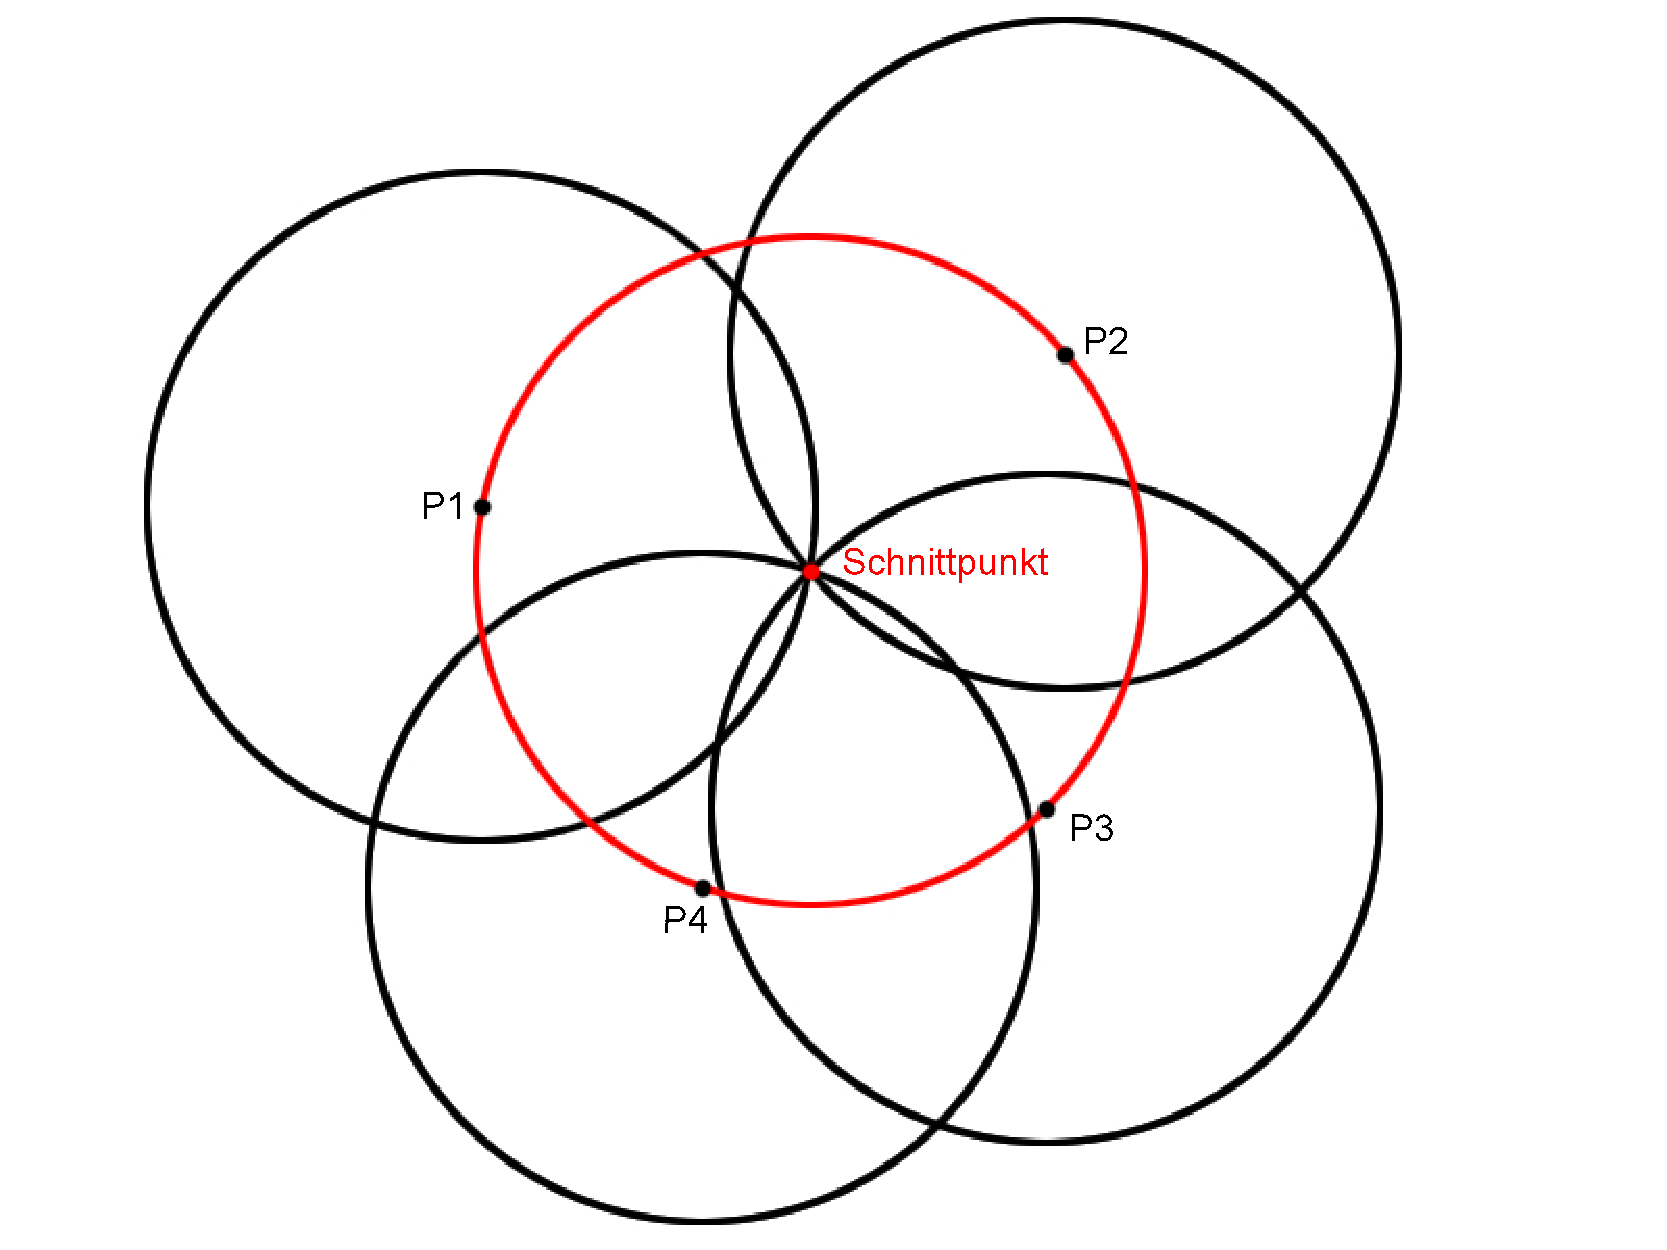
\includegraphics[width=0.5\textwidth]{Bilder/kreise}
\caption{Umgekehrte Heransgehensweise um Punkte auf Kreis zu finden}
\label{img:kreise}
\end{figure}

Es muss somit also nur geschaut werden, ob es bei verschiedenen Radien Schnittpunkte gibt, in denen sich mehr als drei Kreise treffen. Die jeweiligen Schnittpunkte und Radien werden dann vom Algorithmus zurückgegeben und grafisch dargestellt.\\
Der Algorithmus erstellt hierfür zunächst ein Array, welches von den Proportionen der Größe des Sichtbereiches entspricht. Die Kreise werden dann diskretisiert um die jeweiligen Punkte in das Array übertragen. Die Punkte sind hierbei vorher ebenfalls diskretisiert und auf die Größe des Arrays angepasst worden.\\
Die Kreise werden nicht einfach nur „gezeichnet“, sondern es wird im Array, welches vom Typ Integer ist, an jeder Position an der sich der Kreis befindet um Eins inkrementiert. Ein Kreis ist also zunächst durch eine diskrete Anordnung von Einsen im Array dargestellt. Wird nun ein Kreis um einen weiteren Punkt eingezeichnet, der mit dem vorherigen Kreis einen Schnittpunkt hat, so ergibt sich an dem Schnittpunkt im Array ein Wert von Zwei. Sind alle Kreise eingezeichnet worden muss so am Ende nur im Array nach allen Werten gesucht werden, die größer als drei sind. Hier befindet sich ein Schnittpunkt von mehr als drei Kreisen mit dem betrachteten Radius.

\begin{figure}[h]
\centering
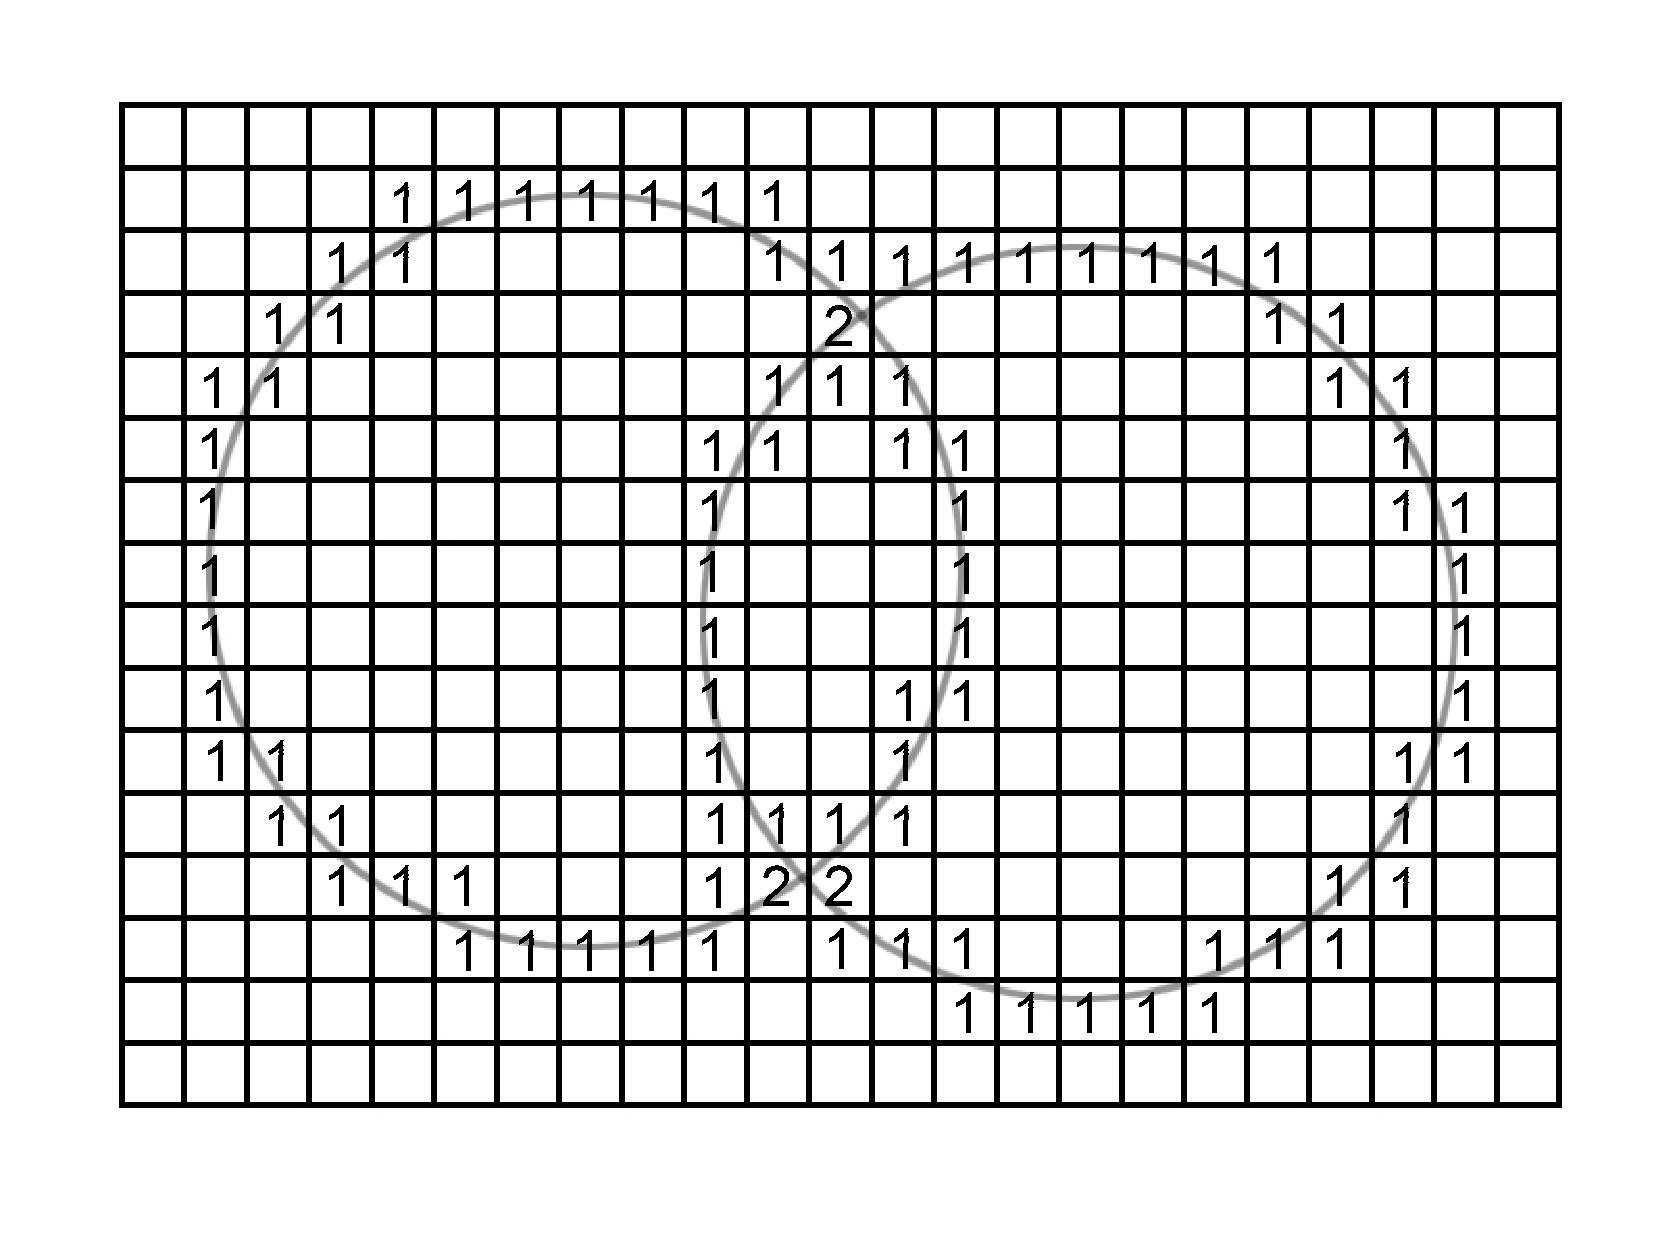
\includegraphics[width=0.5\textwidth]{Bilder/diskret}
\caption{Überscheidung von zwei diskretisierten Kreisen im Array}
\label{img:diskret}
\end{figure}

Die Genauigkeit mit der die Punkte auf einem Kreis liegen lassen sich im Algorithmus über die Größe des Arrays bestimmen. Je größer das Array, desto genauer liegen die Punkte am Ende auf dem Kreis. Hier wurde eine relativ kleine Größe des Array gewählt, sodass Punkte auch dann als auf dem Kreis liegend bewertet werden, wenn sie sich etwas daneben befinden.\\
Als Score ließe sich hier der Abstand der Punkte zu einer möglichen Lage auf einem Kreis angeben. In diesem Projekt wurde jedoch nur überprüft, ob sich mehr als drei Punkte mit einer gewissen Unschärfe auf einem Kreis befinden.












\end{document}
